\documentclass{article}

% content/resources/templates/preamble.tex
\usepackage[margin=0.6in]{geometry}
\author{Milav Dabgar}
\usepackage{amsmath,amssymb,amsthm}
\usepackage{booktabs}
\usepackage{multirow}
\usepackage{xcolor}
\usepackage{tcolorbox}
\tcbuselibrary{breakable,skins}
\usepackage[colorlinks=true,linkcolor=blue]{hyperref}
\usepackage{titlesec}
\usepackage{enumitem}
\usepackage{tikz}
\usepackage{pgfplots}
\usepackage{circuitikz}
\usepackage[version=4]{mhchem}
\usepackage{longtable}
\usepackage{array}
\usepackage{float}
\usepackage{caption}
\usepackage{listings}

\lstset{
  basicstyle=\small\ttfamily,
  breaklines=true,
  breakatwhitespace=false,
  postbreak=\mbox{\textcolor{red}{$\hookrightarrow$}\space},
  float=false,
  numbers=left,
  numberstyle=\tiny\color{gray},
  numbersep=10pt,
  xleftmargin=2em,
  keywordstyle=\color{blue},
  commentstyle=\color{green!60!black},
  stringstyle=\color{purple},
  backgroundcolor=\color{gray!5},
  showstringspaces=false,
  tabsize=2,
  captionpos=b,
  keepspaces=true,
  columns=flexible
}

\pgfplotsset{compat=1.18}
\usetikzlibrary{shapes,arrows,positioning,calc,patterns,decorations.pathmorphing,decorations.markings,arrows.meta}

% Color scheme
\definecolor{headcolor}{RGB}{0,102,204}
\definecolor{keycolor}{RGB}{220,20,60}
\definecolor{solutioncolor}{RGB}{34,139,34}
\definecolor{mnemoniccolor}{RGB}{148,0,211}
\definecolor{codecolor}{RGB}{0,0,100}

% Spacing
\setlength{\parskip}{3pt}
\setlist[itemize]{nosep}
\setlist[enumerate]{nosep}

% Title formatting
\titleformat{\section}{\Large\bfseries\color{headcolor}}{\thesection}{1em}{}
\titleformat{\subsection}{\large\bfseries\color{headcolor}}{\thesubsection}{1em}{}

% Pandoc tightlist compatibility
\providecommand{\tightlist}{%
  \setlength{\itemsep}{0pt}\setlength{\parskip}{0pt}}

% Pandoc longtable compatibility
\newcounter{none}
\def\thenone{}


% content/resources/templates/english-boxes.tex

% Custom environments
\newtcolorbox{solutionbox}{
 breakable,
 enhanced,
 colback=solutioncolor!5!white,
 colframe=solutioncolor!75!black,
 fonttitle=\bfseries,
 title=Solution
}

\newtcolorbox{solutionboxnobreak}{
 colback=solutioncolor!5!white,
 colframe=solutioncolor!75!black,
 fonttitle=\bfseries,
 title=Solution
}

\newtcolorbox{keyformula}{
 breakable,
 enhanced,
 colback=keycolor!5!white,
 colframe=keycolor!75!black,
 fonttitle=\bfseries,
 title=Key Formula
}

\newtcolorbox{mnemonicboxenv}{
 breakable,
 enhanced,
 colback=mnemoniccolor!5!white,
 colframe=mnemoniccolor!75!black,
 fonttitle=\bfseries,
 title=Mnemonic
}

\newcommand{\mnemonicbox}[1]{%
  \begin{mnemonicboxenv}
    #1
  \end{mnemonicboxenv}
}


% Custom commands for GTU solutions
% This file defines semantic commands for consistent formatting

% Question command with automatic formatting
\newcommand{\question}[2]{%
  \section*{Question #1}%
  \textbf{#2}%
}

% OR question variant
\newcommand{\questionor}[2]{%
  \section*{Question #1 OR}%
  \textbf{#2}%
}

% Proper table environment with caption
\newenvironment{answertable}[1]{%
  \begin{table}[htbp]
  \centering
  \caption{#1}
}{%
  \end{table}
}

% Proper figure environment for diagrams
\newenvironment{answerdiagram}[1]{%
  \begin{figure}[htbp]
  \centering
  \caption{#1}
}{%
  \end{figure}
}

% Semantic markup for key terms
\newcommand{\keyword}[1]{\textbf{#1}}
\newcommand{\code}[1]{\texttt{#1}}
\newcommand{\classname}[1]{\texttt{#1}}
\newcommand{\methodname}[1]{\texttt{#1}}

% Proper quotation marks
\newcommand{\mnemonic}[1]{``#1''}


\title{Computer Networks \& Data Communication (4361101) - Winter 2024 Solution}
\date{November 19, 2024}

\begin{document}
\maketitle

\questionmarks{1(a)}{3}{Explain star topology in detail.}

\begin{solutionbox}
Star topology connects all devices to a central hub or switch. Each device has dedicated point-to-point connection with central device.

\textbf{Diagram:}

\begin{figure}[H]
\centering
\begin{tikzpicture}[node distance=2cm, auto]
    \node (hub) [gtu block, circle, minimum size=1.5cm] {HUB};
    \node (pc1) [gtu block, above=of hub] {Computer A};
    \node (pc2) [gtu block, right=of hub] {Computer B};
    \node (pc3) [gtu block, below=of hub] {Computer C};
    \node (pc4) [gtu block, left=of hub] {Computer D};
    
    \draw[gtu arrow] (hub) -- (pc1);
    \draw[gtu arrow] (hub) -- (pc2);
    \draw[gtu arrow] (hub) -- (pc3);
    \draw[gtu arrow] (hub) -- (pc4);
\end{tikzpicture}
\caption{Star Topology}
\end{figure}

\textbf{Key Features:}

\begin{itemize}
    \item \textbf{Central Hub}: All connections pass through central device
    \item \textbf{Dedicated Links}: Each node has separate connection
    \item \textbf{Easy Management}: Simple to add/remove devices
\end{itemize}

\end{solutionbox}

\begin{mnemonicbox}
\mnemonic{Star Shines Central - All devices connect to central point}
\end{mnemonicbox}

\questionmarks{1(b)}{4}{Explain client-server network.}

\begin{solutionbox}
Client-server is network architecture where clients request services from centralized servers. Server provides resources and services to multiple clients.

\textbf{Table: Client vs Server}

\begin{table}[H]
\centering
\begin{tabulary}{\textwidth}{L L}
\toprule
\textbf{Client} & \textbf{Server} \\
\midrule
Requests services & Provides services \\
Limited resources & Powerful hardware \\
Depends on server & Independent operation \\
\bottomrule
\end{tabulary}
\caption{Client vs Server}
\end{table}

\textbf{Key Components:}

\begin{itemize}
    \item \textbf{Client}: Requests data/services from server
    \item \textbf{Server}: Provides centralized resources and processing
    \item \textbf{Network}: Medium for communication between client-server
\end{itemize}

\end{solutionbox}

\begin{mnemonicbox}
\mnemonic{Client Calls, Server Serves}
\end{mnemonicbox}

\questionmarks{1(c)}{7}{Write a functional description of all layer of TCP/IP model.}

\begin{solutionbox}
TCP/IP model has four layers providing end-to-end communication over networks.

\textbf{Table: TCP/IP Model Layers}

\begin{table}[H]
\centering
\begin{tabulary}{\textwidth}{L L L}
\toprule
\textbf{Layer} & \textbf{Function} & \textbf{Protocols} \\
\midrule
Application & User interface, network services & HTTP, FTP, SMTP \\
Transport & End-to-end delivery, error control & TCP, UDP \\
Internet & Routing, logical addressing & IP, ICMP, ARP \\
Network Access & Physical transmission & Ethernet, WiFi \\
\bottomrule
\end{tabulary}
\caption{TCP/IP Model Layers}
\end{table}

\textbf{Layer Functions:}

\begin{itemize}
    \item \textbf{Application Layer}: Provides network services to user applications
    \item \textbf{Transport Layer}: Ensures reliable data delivery between processes
    \item \textbf{Internet Layer}: Routes packets across multiple networks using IP
    \item \textbf{Network Access Layer}: Handles physical transmission of data
\end{itemize}

\end{solutionbox}

\begin{mnemonicbox}
\mnemonic{All Transport Internet Networks (ATIN)}
\end{mnemonicbox}

\questionmarks{1(c OR)}{7}{Explain the functions of Data Link Layer \& Network Layer of OSI reference model.}

\begin{solutionbox}
Data Link and Network layers provide reliable transmission and routing capabilities in OSI model.

\textbf{Table: Layer Comparison}

\begin{table}[H]
\centering
\begin{tabulary}{\textwidth}{L L L}
\toprule
\textbf{Feature} & \textbf{Data Link Layer} & \textbf{Network Layer} \\
\midrule
Main Function & Node-to-node delivery & End-to-end delivery \\
Addressing & MAC addresses & IP addresses \\
Error Control & Frame-level & Packet-level \\
\bottomrule
\end{tabulary}
\caption{Layer Comparison}
\end{table}

\textbf{Data Link Layer Functions:}

\begin{itemize}
    \item \textbf{Framing}: Organizes bits into frames
    \item \textbf{Error Control}: Detects and corrects transmission errors
    \item \textbf{Flow Control}: Manages data transmission rate
\end{itemize}

\textbf{Network Layer Functions:}

\begin{itemize}
    \item \textbf{Routing}: Determines best path for packets
    \item \textbf{Logical Addressing}: Uses IP addresses for identification
    \item \textbf{Packet Forwarding}: Routes packets between networks
\end{itemize}

\end{solutionbox}

\begin{mnemonicbox}
\mnemonic{Data Links Locally, Network Routes Globally}
\end{mnemonicbox}

\questionmarks{2(a)}{3}{Compare repeater and hub.}

\begin{solutionbox}
Both devices amplify signals but operate differently in network architecture.

\textbf{Table: Repeater vs Hub}

\begin{table}[H]
\centering
\begin{tabulary}{\textwidth}{L L L}
\toprule
\textbf{Feature} & \textbf{Repeater} & \textbf{Hub} \\
\midrule
Ports & 2 ports & Multiple ports \\
Function & Signal amplification & Signal distribution \\
Collision Domain & Single & Single shared \\
\bottomrule
\end{tabulary}
\caption{Repeater vs Hub}
\end{table}

\textbf{Key Differences:}

\begin{itemize}
    \item \textbf{Port Count}: Repeater has 2 ports, hub has multiple
    \item \textbf{Usage}: Repeater extends distance, hub connects multiple devices
\end{itemize}

\end{solutionbox}

\begin{mnemonicbox}
\mnemonic{Repeater Extends, Hub Connects}
\end{mnemonicbox}

\questionmarks{2(b)}{4}{Explain wireless LAN.}

\begin{solutionbox}
Wireless LAN uses radio waves for network communication without physical cables.

\textbf{Diagram:}

\begin{figure}[H]
\centering
\begin{tikzpicture}[node distance=2.5cm, auto]
    \node (ap) [gtu block, circle, minimum size=1.5cm, fill=blue!10] {Access Point};
    \node (laptop) [gtu block, above left=of ap] {Laptop};
    \node (desktop) [gtu block, above right=of ap] {Desktop};
    \node (mobile) [gtu block, below left=of ap] {Mobile};
    \node (printer) [gtu block, below right=of ap] {Printer};
    
    \draw[dashed, gtu arrow, <->] (ap) -- (laptop) node[midway, sloped, above, font=\tiny] {WiFi};
    \draw[dashed, gtu arrow, <->] (ap) -- (desktop) node[midway, sloped, above, font=\tiny] {WiFi};
    \draw[dashed, gtu arrow, <->] (ap) -- (mobile) node[midway, sloped, above, font=\tiny] {WiFi};
    \draw[dashed, gtu arrow, <->] (ap) -- (printer) node[midway, sloped, above, font=\tiny] {WiFi};
\end{tikzpicture}
\caption{Wireless LAN Architecture}
\end{figure}

\textbf{Key Components:}

\begin{itemize}
    \item \textbf{Access Point}: Central wireless communication device
    \item \textbf{Wireless Clients}: Devices with WiFi capability
    \item \textbf{Radio Frequencies}: 2.4GHz and 5GHz bands commonly used
\end{itemize}

\textbf{Advantages:}

\begin{itemize}
    \item \textbf{Mobility}: Users can move freely within coverage area
    \item \textbf{Easy Installation}: No physical cable installation required
\end{itemize}

\end{solutionbox}

\begin{mnemonicbox}
\mnemonic{Wireless Waves Connect}
\end{mnemonicbox}

\questionmarks{2(c)}{7}{Explain FDDI \& CDDI.}

\begin{solutionbox}
FDDI and CDDI are ring-based network technologies providing high-speed data transmission.

\textbf{Table: FDDI vs CDDI Comparison}

\begin{table}[H]
\centering
\begin{tabulary}{\textwidth}{L L L}
\toprule
\textbf{Feature} & \textbf{FDDI} & \textbf{CDDI} \\
\midrule
Medium & Fiber optic & Copper (UTP) \\
Speed & 100 Mbps & 100 Mbps \\
Distance & 200 km & 100 meters \\
Cost & High & Lower \\
\bottomrule
\end{tabulary}
\caption{FDDI vs CDDI}
\end{table}

\textbf{FDDI Features:}

\begin{itemize}
    \item \textbf{Dual Ring}: Primary and secondary rings for fault tolerance
    \item \textbf{Token Passing}: Deterministic access method
    \item \textbf{Self-Healing}: Automatic recovery from failures
\end{itemize}

\textbf{CDDI Features:}

\begin{itemize}
    \item \textbf{Copper Medium}: Uses unshielded twisted pair cables
    \item \textbf{Same Protocol}: Identical to FDDI except transmission medium
    \item \textbf{Cost Effective}: Lower implementation cost than FDDI
\end{itemize}

\textbf{Ring Structure:}

\begin{figure}[H]
\centering
\begin{tikzpicture}[node distance=2.5cm, auto]
    \node (sta) [gtu block] {Station A};
    \node (stb) [gtu block, right=of sta] {Station B};
    \node (stc) [gtu block, below=of stb] {Station C};
    \node (std) [gtu block, left=of stc] {Station D};
    
    % Primary Ring
    \draw[->, thick, blue] (sta) -- (stb);
    \draw[->, thick, blue] (stb) -- (stc);
    \draw[->, thick, blue] (stc) -- (std);
    \draw[->, thick, blue] (std) -- (sta);
    
    % Secondary Ring (Dashed, Counter-rotating)
    \draw[->, dashed, red] (stb) to[bend right=15] (sta);
    \draw[->, dashed, red] (sta) to[bend right=15] (std);
    \draw[->, dashed, red] (std) to[bend right=15] (stc);
    \draw[->, dashed, red] (stc) to[bend right=15] (stb);
    
    \node[align=center, font=\footnotesize] at (3.5, -1.5) {Blue: Primary Ring\\Red: Secondary Ring};
\end{tikzpicture}
\caption{FDDI Dual Ring Topology}
\end{figure}

\end{solutionbox}

\begin{mnemonicbox}
\mnemonic{FDDI Fiber Fast, CDDI Copper Cheap}
\end{mnemonicbox}

\questionmarks{2(a OR)}{3}{How does a firewall protect data.}

\begin{solutionbox}
Firewall acts as security barrier between trusted internal network and untrusted external networks.

\textbf{Protection Methods:}

\begin{itemize}
    \item \textbf{Packet Filtering}: Examines packet headers for security rules
    \item \textbf{Access Control}: Blocks unauthorized access attempts
    \item \textbf{Traffic Monitoring}: Monitors all incoming and outgoing traffic
\end{itemize}

\end{solutionbox}

\begin{mnemonicbox}
\mnemonic{Firewall Filters Foes}
\end{mnemonicbox}

\questionmarks{2(b OR)}{4}{Explain the structure of FDDI and give its advantages.}

\begin{solutionbox}
FDDI uses dual counter-rotating rings for high-speed, fault-tolerant networking.

\textbf{Structure Components:}

\begin{itemize}
    \item \textbf{Primary Ring}: Main data transmission path
    \item \textbf{Secondary Ring}: Backup path for fault recovery
    \item \textbf{Dual Attachment Stations}: Connect to both rings
    \item \textbf{Single Attachment Stations}: Connect to one ring only
\end{itemize}

\textbf{Advantages:}

\begin{itemize}
    \item \textbf{High Speed}: 100 Mbps transmission rate
    \item \textbf{Fault Tolerance}: Automatic recovery using secondary ring
    \item \textbf{Long Distance}: Supports up to 200 km networks
\end{itemize}

\end{solutionbox}

\begin{mnemonicbox}
\mnemonic{FDDI Dual Rings Deliver Reliability}
\end{mnemonicbox}

\questionmarks{2(c OR)}{7}{Explain and distinguish Ethernet, Fast Ethernet, Gigabit Ethernet.}

\begin{solutionbox}
Evolution of Ethernet standards providing increasing bandwidth and improved performance.

\textbf{Table: Ethernet Comparison}

\begin{table}[H]
\centering
\begin{tabulary}{\textwidth}{L L L L}
\toprule
\textbf{Feature} & \textbf{Ethernet} & \textbf{Fast Ethernet} & \textbf{Gigabit Ethernet} \\
\midrule
Speed & 10 Mbps & 100 Mbps & 1000 Mbps \\
Standard & 802.3 & 802.3u & 802.3z/ab \\
Cable & Coax/UTP & UTP/Fiber & UTP/Fiber \\
Distance & 500m (coax) & 100m (UTP) & 100m (UTP) \\
\bottomrule
\end{tabulary}
\caption{Ethernet Comparison}
\end{table}

\textbf{Key Differences:}

\begin{itemize}
    \item \textbf{Bandwidth}: Each generation increases speed by factor of 10
    \item \textbf{Media Support}: Newer standards support more cable types
    \item \textbf{Backward Compatibility}: Higher standards support lower speeds
\end{itemize}

\textbf{Applications:}

\begin{itemize}
    \item \textbf{Ethernet}: Legacy systems, basic connectivity
    \item \textbf{Fast Ethernet}: Desktop connections, small networks
    \item \textbf{Gigabit Ethernet}: Server connections, backbone networks
\end{itemize}

\end{solutionbox}

\begin{mnemonicbox}
\mnemonic{Ethernet Evolves: 10-100-1000}
\end{mnemonicbox}

\questionmarks{3(a)}{3}{Explain types of DSL.}

\begin{solutionbox}
DSL provides high-speed internet over existing telephone lines using different frequency bands.

\textbf{Table: DSL Types}

\begin{table}[H]
\centering
\begin{tabulary}{\textwidth}{L L L}
\toprule
\textbf{Type} & \textbf{Full Form} & \textbf{Speed} \\
\midrule
ADSL & Asymmetric DSL & Up to 8 Mbps down \\
SDSL & Symmetric DSL & Equal up/down \\
VDSL & Very-high-bit-rate DSL & Up to 52 Mbps \\
\bottomrule
\end{tabulary}
\caption{DSL Types}
\end{table}

\textbf{Characteristics:}

\begin{itemize}
    \item \textbf{ADSL}: Different upload/download speeds for home users
    \item \textbf{SDSL}: Same speed both directions for business use
\end{itemize}

\end{solutionbox}

\begin{mnemonicbox}
\mnemonic{DSL: Asymmetric, Symmetric, Very-fast}
\end{mnemonicbox}

\questionmarks{3(b)}{4}{Explain ARP \& RARP.}

\begin{solutionbox}
ARP and RARP provide address resolution between IP and MAC addresses.

\textbf{Table: ARP vs RARP}

\begin{table}[H]
\centering
\begin{tabulary}{\textwidth}{L L L}
\toprule
\textbf{Feature} & \textbf{ARP} & \textbf{RARP} \\
\midrule
Purpose & IP to MAC & MAC to IP \\
Used by & All devices & Diskless workstations \\
Direction & Logical to Physical & Physical to Logical \\
\bottomrule
\end{tabulary}
\caption{ARP vs RARP}
\end{table}

\textbf{ARP Process:}

\begin{itemize}
    \item \textbf{Request}: Broadcast "Who has IP address X?"
    \item \textbf{Reply}: Target responds with MAC address
    \item \textbf{Caching}: Stores mapping in ARP table
\end{itemize}

\textbf{RARP Process:}

\begin{itemize}
    \item \textbf{Request}: "What is my IP address?"
    \item \textbf{Server Response}: RARP server provides IP address
\end{itemize}

\end{solutionbox}

\begin{mnemonicbox}
\mnemonic{ARP: Address Resolution Protocol, RARP: Reverse ARP}
\end{mnemonicbox}

\questionmarks{3(c)}{7}{Describe circuit switching and packet switching.}

\begin{solutionbox}
Two fundamental approaches for establishing communication paths in networks.

\textbf{Table: Circuit vs Packet Switching}

\begin{table}[H]
\centering
\begin{tabulary}{\textwidth}{L L L}
\toprule
\textbf{Feature} & \textbf{Circuit Switching} & \textbf{Packet Switching} \\
\midrule
Path Setup & Dedicated path & No dedicated path \\
Resource Usage & Reserved throughout & Shared dynamically \\
Delay & Constant & Variable \\
Examples & Telephone & Internet \\
\bottomrule
\end{tabulary}
\caption{Circuit vs Packet Switching}
\end{table}

\textbf{Circuit Switching:}

\begin{itemize}
    \item \textbf{Path Establishment}: Dedicated circuit created before communication
    \item \textbf{Resource Reservation}: Bandwidth reserved for entire session
    \item \textbf{Guaranteed Service}: Consistent performance throughout connection
\end{itemize}

\textbf{Packet Switching:}

\begin{itemize}
    \item \textbf{Store and Forward}: Packets stored temporarily at intermediate nodes
    \item \textbf{Dynamic Routing}: Each packet can take different path
    \item \textbf{Resource Sharing}: Network resources shared among multiple connections
\end{itemize}

\textbf{Diagram: Packet Switching}

\begin{figure}[H]
\centering
\begin{tikzpicture}[node distance=2.5cm, auto]
    \node (src) [gtu block] {Source};
    \node (r1) [gtu block, circle, minimum size=1cm, right=of src] {R1};
    \node (r2) [gtu block, circle, minimum size=1cm, right=of r1] {R2};
    \node (r3) [gtu block, circle, minimum size=1cm, below=of r1] {R3};
    \node (dest) [gtu block, right=of r2] {Destination};

    \draw[gtu arrow] (src) -- (r1);
    \draw[gtu arrow] (r1) -- (r2);
    \draw[gtu arrow] (r2) -- (dest);
    \draw[gtu arrow] (src) -- (r3);
    \draw[gtu arrow] (r3) -- (r2);
    
    \node [font=\small] at (3,-1.5) {Packets take different paths};
\end{tikzpicture}
\caption{Packet Switching}
\end{figure}

\end{solutionbox}

\begin{mnemonicbox}
\mnemonic{Circuit Commits, Packet Partitions}
\end{mnemonicbox}

\questionmarks{3(a OR)}{3}{Describe DHCP \& BOOTP protocol.}

\begin{solutionbox}
Both protocols automatically assign IP addresses to network devices.

\textbf{Table: DHCP vs BOOTP}

\begin{table}[H]
\centering
\begin{tabulary}{\textwidth}{L L L}
\toprule
\textbf{Feature} & \textbf{DHCP} & \textbf{BOOTP} \\
\midrule
Address Type & Dynamic/Static & Static only \\
Lease Time & Temporary & Permanent \\
Configuration & Automatic & Manual setup \\
\bottomrule
\end{tabulary}
\caption{DHCP vs BOOTP}
\end{table}

\textbf{Functions:}

\begin{itemize}
    \item \textbf{DHCP}: Dynamic address assignment with lease management
    \item \textbf{BOOTP}: Bootstrap protocol for diskless workstations
\end{itemize}

\end{solutionbox}

\begin{mnemonicbox}
\mnemonic{DHCP Dynamic, BOOTP Bootstrap}
\end{mnemonicbox}

\questionmarks{3(b OR)}{4}{Explain IPv4 \& IPv6 in detail.}

\begin{solutionbox}
Internet Protocol versions providing addressing and routing capabilities.

\textbf{Table: IPv4 vs IPv6}

\begin{table}[H]
\centering
\begin{tabulary}{\textwidth}{L L L}
\toprule
\textbf{Feature} & \textbf{IPv4} & \textbf{IPv6} \\
\midrule
Address Size & 32 bits & 128 bits \\
Address Format & Dotted decimal & Hexadecimal \\
Address Space & 4.3 billion & 340 undecillion \\
Header Size & 20-60 bytes & 40 bytes \\
\bottomrule
\end{tabulary}
\caption{IPv4 vs IPv6}
\end{table}

\textbf{IPv4 Features:}

\begin{itemize}
    \item \textbf{Address Format}: 192.168.1.1 (4 octets)
    \item \textbf{Classes}: A, B, C, D, E address classes
    \item \textbf{NAT Required}: Address shortage requires NAT
\end{itemize}

\textbf{IPv6 Features:}

\begin{itemize}
    \item \textbf{Address Format}: 2001:db8::1 (8 groups of 4 hex digits)
    \item \textbf{No NAT Needed}: Abundant address space
    \item \textbf{Built-in Security}: IPSec support mandatory
\end{itemize}

\end{solutionbox}

\begin{mnemonicbox}
\mnemonic{IPv4 Four Octets, IPv6 Six-teen Bytes}
\end{mnemonicbox}

\questionmarks{3(c OR)}{7}{Draw and explain constructional details of twisted pair cable, coaxial cable, and fiber optic cable with label.}

\begin{solutionbox}
Three main types of guided transmission media with different construction and characteristics.

\textbf{Twisted Pair Cable:}

\begin{figure}[H]
\centering
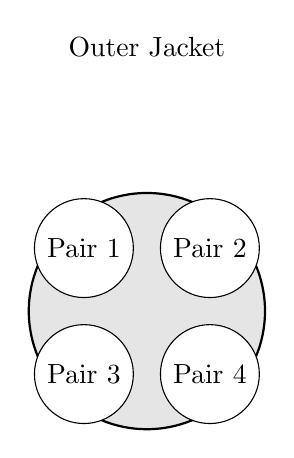
\begin{tikzpicture}[auto]
    \node (jacket) [circle, draw, minimum size=3cm, thick, fill=gray!20] {};
    \node (pair1) [circle, draw, minimum size=0.8cm, fill=white] at (-0.8,0.8) {Pair 1};
    \node (pair2) [circle, draw, minimum size=0.8cm, fill=white] at (0.8,0.8) {Pair 2};
    \node (pair3) [circle, draw, minimum size=0.8cm, fill=white] at (-0.8,-0.8) {Pair 3};
    \node (pair4) [circle, draw, minimum size=0.8cm, fill=white] at (0.8,-0.8) {Pair 4};
    \node [above=1.6cm of jacket] {Outer Jacket};
\end{tikzpicture}
\caption{Twisted Pair Cable Cross-section}
\end{figure}

\textbf{Coaxial Cable:}

\begin{figure}[H]
\centering
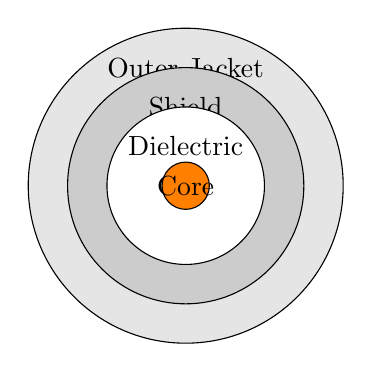
\begin{tikzpicture}[auto]
    \draw[fill=black!10] (0,0) circle (2cm); \node at (0,1.5) {Outer Jacket};
    \draw[fill=gray!40] (0,0) circle (1.5cm); \node at (0,1) {Shield};
    \draw[fill=white] (0,0) circle (1cm); \node at (0,0.5) {Dielectric};
    \draw[fill=orange] (0,0) circle (0.3cm); \node at (0,0) {Core};
\end{tikzpicture}
\caption{Coaxial Cable Cross-section}
\end{figure}

\textbf{Fiber Optic Cable:}

\begin{figure}[H]
\centering
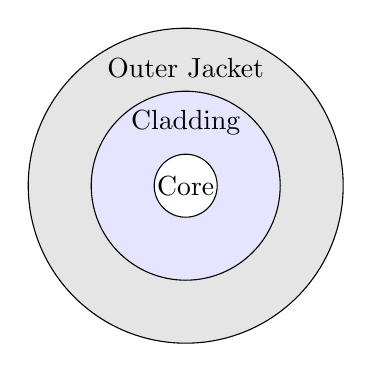
\begin{tikzpicture}[auto]
    \draw[fill=black!10] (0,0) circle (2cm); \node at (0,1.5) {Outer Jacket};
    \draw[fill=blue!10] (0,0) circle (1.2cm); \node at (0,0.8) {Cladding};
    \draw[fill=white] (0,0) circle (0.4cm); \node at (0,0) {Core};
\end{tikzpicture}
\caption{Fiber Optic Cable Cross-section}
\end{figure}

\textbf{Construction Details:}

\begin{itemize}
    \item \textbf{Twisted Pair}: Copper wires twisted to reduce interference
    \item \textbf{Coaxial}: Central conductor surrounded by dielectric and shield
    \item \textbf{Fiber Optic}: Glass core with cladding for total internal reflection
\end{itemize}

\textbf{Characteristics:}

\begin{itemize}
    \item \textbf{Twisted Pair}: Low cost, easy installation, limited bandwidth
    \item \textbf{Coaxial}: Better shielding, higher bandwidth than twisted pair
    \item \textbf{Fiber Optic}: Highest bandwidth, immune to electromagnetic interference
\end{itemize}

\end{solutionbox}

\begin{mnemonicbox}
\mnemonic{Twisted Copper, Coax Shielded, Fiber Light}
\end{mnemonicbox}

\questionmarks{4(a)}{3}{Name any three data link layer protocol and explain any one in detail.}

\begin{solutionbox}
Common data link layer protocols: HDLC, PPP, Ethernet.

\textbf{HDLC (High-Level Data Link Control):}

\begin{itemize}
    \item \textbf{Frame Structure}: Flag, Address, Control, Data, FCS, Flag
    \item \textbf{Error Control}: Uses sequence numbers and acknowledgments
    \item \textbf{Flow Control}: Sliding window protocol for efficient transmission
\end{itemize}

\textbf{Key Features:}

\begin{itemize}
    \item \textbf{Bit-oriented}: Works with bit streams rather than characters
    \item \textbf{Full-duplex}: Simultaneous bidirectional communication
\end{itemize}

\end{solutionbox}

\begin{mnemonicbox}
\mnemonic{HDLC Handles Data Link Control}
\end{mnemonicbox}

\questionmarks{4(b)}{4}{Explain TCP and UDP protocol.}

\begin{solutionbox}
Transport layer protocols providing different levels of service reliability.

\textbf{Table: TCP vs UDP}

\begin{table}[H]
\centering
\begin{tabulary}{\textwidth}{L L L}
\toprule
\textbf{Feature} & \textbf{TCP} & \textbf{UDP} \\
\midrule
Connection & Connection-oriented & Connectionless \\
Reliability & Reliable & Unreliable \\
Speed & Slower & Faster \\
Header Size & 20+ bytes & 8 bytes \\
\bottomrule
\end{tabulary}
\caption{TCP vs UDP}
\end{table}

\textbf{TCP Features:}

\begin{itemize}
    \item \textbf{Connection Setup}: Three-way handshake establishes connection
    \item \textbf{Error Recovery}: Retransmits lost packets automatically
    \item \textbf{Flow Control}: Prevents sender from overwhelming receiver
\end{itemize}

\textbf{UDP Features:}

\begin{itemize}
    \item \textbf{No Connection}: Sends data without establishing connection
    \item \textbf{Best Effort}: No guarantee of delivery or order
    \item \textbf{Low Overhead}: Minimal header for fast transmission
\end{itemize}

\end{solutionbox}

\begin{mnemonicbox}
\mnemonic{TCP Trustworthy, UDP Unreliable but Quick}
\end{mnemonicbox}

\questionmarks{4(c)}{7}{Describe VoIP with example.}

\begin{solutionbox}
Voice over Internet Protocol transmits voice communications over IP networks instead of traditional telephone systems.

\textbf{VoIP Components:}

\begin{itemize}
    \item \textbf{IP Phone}: Hardware device for VoIP calls
    \item \textbf{Softphone}: Software application for computer-based calls
    \item \textbf{Gateway}: Connects VoIP to traditional phone networks
    \item \textbf{PBX}: Private branch exchange for business phone systems
\end{itemize}

\textbf{VoIP Process:}

\begin{enumerate}
    \item \textbf{Voice Capture}: Microphone converts voice to analog signal
    \item \textbf{Digitization}: ADC converts analog to digital samples
    \item \textbf{Compression}: Codec compresses audio data
    \item \textbf{Packetization}: Voice data divided into IP packets
    \item \textbf{Transmission}: Packets sent over IP network
    \item \textbf{Reconstruction}: Receiving end reassembles and plays audio
\end{enumerate}

\textbf{Example Applications:}

\begin{itemize}
    \item \textbf{Skype}: Consumer VoIP service for personal calls
    \item \textbf{WhatsApp Calling}: Mobile VoIP application
    \item \textbf{Business PBX}: Corporate phone systems using VoIP
\end{itemize}

\textbf{Advantages:}

\begin{itemize}
    \item \textbf{Cost Effective}: Lower long-distance call costs
    \item \textbf{Feature Rich}: Video calling, conferencing, call forwarding
    \item \textbf{Scalability}: Easy to add new users
\end{itemize}

\textbf{Disadvantages:}

\begin{itemize}
    \item \textbf{Internet Dependency}: Requires stable internet connection
    \item \textbf{Quality Issues}: May suffer from network congestion
    \item \textbf{Power Dependency}: Requires electricity unlike traditional phones
\end{itemize}

\end{solutionbox}

\begin{mnemonicbox}
\mnemonic{VoIP: Voice over Internet Protocol}
\end{mnemonicbox}

\questionmarks{4(a OR)}{3}{Explain DNS (Domain Name System).}

\begin{solutionbox}
DNS translates human-readable domain names into IP addresses for network communication.

\textbf{DNS Components:}

\begin{itemize}
    \item \textbf{Domain Names}: Hierarchical naming system (www.example.com)
    \item \textbf{Name Servers}: Computers that store DNS records
    \item \textbf{Resolvers}: Client software that queries DNS servers
\end{itemize}

\textbf{DNS Process:}

\begin{enumerate}
    \item User enters domain name in browser
    \item Local resolver queries DNS server
    \item DNS server returns corresponding IP address
\end{enumerate}

\end{solutionbox}

\begin{mnemonicbox}
\mnemonic{DNS: Domain Name to IP Address}
\end{mnemonicbox}

\questionmarks{4(b OR)}{4}{Write a short note on DSL.}

\begin{solutionbox}
Digital Subscriber Line provides high-speed internet access over existing telephone infrastructure.

\textbf{DSL Technology:}

\begin{itemize}
    \item \textbf{Frequency Division}: Uses higher frequencies than voice calls
    \item \textbf{Simultaneous Use}: Internet and phone can work together
    \item \textbf{Distance Limitation}: Performance decreases with distance from exchange
\end{itemize}

\textbf{DSL Types:}

\begin{itemize}
    \item \textbf{ADSL}: Asymmetric speeds for residential users
    \item \textbf{SDSL}: Symmetric speeds for business applications
    \item \textbf{VDSL}: Very high speeds over short distances
\end{itemize}

\textbf{Advantages:}

\begin{itemize}
    \item \textbf{Existing Infrastructure}: Uses existing telephone lines
    \item \textbf{Always On}: Continuous internet connection
    \item \textbf{Cost Effective}: Lower cost than dedicated lines
\end{itemize}

\end{solutionbox}

\begin{mnemonicbox}
\mnemonic{DSL: Digital Subscriber Line over Phone Lines}
\end{mnemonicbox}

\questionmarks{4(c OR)}{7}{Explain forum and blogs with example.}

\begin{solutionbox}
Online platforms for information sharing and community interaction.

\textbf{Table: Forum vs Blog}

\begin{table}[H]
\centering
\begin{tabulary}{\textwidth}{L L L}
\toprule
\textbf{Feature} & \textbf{Forum} & \textbf{Blog} \\
\midrule
Structure & Discussion threads & Chronological posts \\
Interaction & Multi-user discussions & Comments on posts \\
Moderation & Community moderated & Author controlled \\
Purpose & Community support & Information sharing \\
\bottomrule
\end{tabulary}
\caption{Forum vs Blog}
\end{table}

\textbf{Forum Characteristics:}

\begin{itemize}
    \item \textbf{Discussion Threads}: Topics organized by subject
    \item \textbf{User Participation}: Multiple users contribute to discussions
    \item \textbf{Categories}: Topics organized into different sections
    \item \textbf{Moderation}: Community rules and moderators maintain order
\end{itemize}

\textbf{Blog Characteristics:}

\begin{itemize}
    \item \textbf{Personal Publishing}: Individual or organization publishes content
    \item \textbf{Chronological Order}: Posts displayed by date
    \item \textbf{Comments}: Readers can respond to blog posts
    \item \textbf{RSS Feeds}: Readers can subscribe to updates
\end{itemize}

\textbf{Examples:}

\begin{itemize}
    \item \textbf{Technical Forums}: Stack Overflow for programming questions
    \item \textbf{Community Forums}: Reddit for diverse topics
    \item \textbf{Personal Blogs}: Individual websites sharing experiences
    \item \textbf{Corporate Blogs}: Company blogs for marketing and updates
\end{itemize}

\textbf{Benefits:}

\begin{itemize}
    \item \textbf{Knowledge Sharing}: Users share expertise and experiences
    \item \textbf{Community Building}: Brings together people with common interests
    \item \textbf{Problem Solving}: Forums help users find solutions
    \item \textbf{Content Creation}: Blogs provide platform for publishing
\end{itemize}

\end{solutionbox}

\begin{mnemonicbox}
\mnemonic{Forums Foster Discussion, Blogs Broadcast Information}
\end{mnemonicbox}

\questionmarks{5(a)}{3}{Define the terms "encryption".}

\begin{solutionbox}
Encryption converts plaintext data into ciphertext to protect information from unauthorized access.

\textbf{Encryption Process:}

\begin{itemize}
    \item \textbf{Plaintext}: Original readable data
    \item \textbf{Algorithm}: Mathematical process for transformation
    \item \textbf{Key}: Secret parameter used in encryption algorithm
    \item \textbf{Ciphertext}: Encrypted unreadable data
\end{itemize}

\textbf{Purpose:}

\begin{itemize}
    \item \textbf{Confidentiality}: Prevents unauthorized data access
    \item \textbf{Data Protection}: Secures sensitive information during transmission
\end{itemize}

\end{solutionbox}

\begin{mnemonicbox}
\mnemonic{Encryption: Plain to Cipher with Key}
\end{mnemonicbox}

\questionmarks{5(b)}{4}{Explain any two of following: (1) WWW (2) FTP (3) SMTP}

\begin{solutionbox}

\textbf{WWW (World Wide Web):}

\begin{itemize}
    \item \textbf{Hypertext System}: Documents linked through hyperlinks
    \item \textbf{HTTP Protocol}: HyperText Transfer Protocol for web communication
    \item \textbf{Web Browser}: Client software for accessing web pages
    \item \textbf{Web Server}: Hosts websites and serves web pages
\end{itemize}

\textbf{FTP (File Transfer Protocol):}

\begin{itemize}
    \item \textbf{File Transfer}: Protocol for transferring files between computers
    \item \textbf{Client-Server}: FTP client connects to FTP server
    \item \textbf{Two Modes}: Active and passive modes for data transfer
    \item \textbf{Authentication}: Username and password for access control
\end{itemize}

\textbf{Features:}

\begin{itemize}
    \item \textbf{WWW}: Graphical interface, multimedia support, hyperlinks
    \item \textbf{FTP}: Large file transfer, directory navigation, resume capability
\end{itemize}

\end{solutionbox}

\begin{mnemonicbox}
\mnemonic{WWW: Web World Wide, FTP: File Transfer Protocol}
\end{mnemonicbox}

\questionmarks{5(c)}{7}{Difference between symmetric and asymmetric encryption algorithms}

\begin{solutionbox}
Two fundamental approaches to cryptographic key management with different characteristics.

\textbf{Table: Symmetric vs Asymmetric Encryption}

\begin{table}[H]
\centering
\begin{tabulary}{\textwidth}{L L L}
\toprule
\textbf{Feature} & \textbf{Symmetric} & \textbf{Asymmetric} \\
\midrule
Keys & Single shared key & Key pair (public/private) \\
Speed & Fast & Slower \\
Key Distribution & Difficult & Easier \\
Key Management & Complex for large groups & Simpler \\
Examples & AES, DES & RSA, ECC \\
\bottomrule
\end{tabulary}
\caption{Symmetric vs Asymmetric Encryption}
\end{table}

\textbf{Symmetric Encryption:}

\begin{itemize}
    \item \textbf{Single Key}: Same key used for encryption and decryption
    \item \textbf{Speed}: Fast processing due to simple algorithms
    \item \textbf{Key Sharing Problem}: Secure key distribution challenge
    \item \textbf{Session Keys}: Often used for bulk data encryption
\end{itemize}

\textbf{Asymmetric Encryption:}

\begin{itemize}
    \item \textbf{Key Pair}: Public key for encryption, private key for decryption
    \item \textbf{Digital Signatures}: Private key signs, public key verifies
    \item \textbf{Key Exchange}: Solves key distribution problem
    \item \textbf{Computationally Intensive}: Slower than symmetric encryption
\end{itemize}

\textbf{Usage Scenarios:}

\begin{itemize}
    \item \textbf{Symmetric}: Bulk data encryption, secure communications
    \item \textbf{Asymmetric}: Key exchange, digital signatures, authentication
\end{itemize}

\textbf{Hybrid Approach:}

\begin{itemize}
    \item \textbf{Best of Both}: Asymmetric for key exchange, symmetric for data
    \item \textbf{SSL/TLS}: Uses both types for secure web communications
\end{itemize}

\end{solutionbox}

\begin{mnemonicbox}
\mnemonic{Symmetric Single Key, Asymmetric Key Pair}
\end{mnemonicbox}

\questionmarks{5(a OR)}{3}{Write brief note on Cyber Security.}

\begin{solutionbox}
Cyber security protects digital systems, networks, and data from digital attacks and unauthorized access.

\textbf{Key Components:}

\begin{itemize}
    \item \textbf{Network Security}: Protects network infrastructure from intrusions
    \item \textbf{Data Protection}: Safeguards sensitive information from theft
    \item \textbf{Application Security}: Secures software applications from vulnerabilities
\end{itemize}

\textbf{Common Threats:}

\begin{itemize}
    \item \textbf{Malware}: Viruses, worms, trojans that damage systems
    \item \textbf{Phishing}: Fraudulent attempts to steal credentials
\end{itemize}

\end{solutionbox}

\begin{mnemonicbox}
\mnemonic{Cyber Security: Protect Digital Assets}
\end{mnemonicbox}

\questionmarks{5(b OR)}{4}{Explain hacking and its precautions.}

\begin{solutionbox}
Hacking involves unauthorized access to computer systems, often with malicious intent.

\textbf{Types of Hacking:}

\begin{itemize}
    \item \textbf{White Hat}: Ethical hacking for security testing
    \item \textbf{Black Hat}: Malicious hacking for illegal purposes
    \item \textbf{Gray Hat}: Between ethical and malicious hacking
\end{itemize}

\textbf{Common Hacking Methods:}

\begin{itemize}
    \item \textbf{Password Attacks}: Brute force, dictionary attacks
    \item \textbf{Social Engineering}: Manipulating people to reveal information
    \item \textbf{Malware}: Viruses, trojans, ransomware
    \item \textbf{Network Attacks}: Man-in-the-middle, packet sniffing
\end{itemize}

\textbf{Precautions:}

\begin{itemize}
    \item \textbf{Strong Passwords}: Complex, unique passwords for all accounts
    \item \textbf{Regular Updates}: Keep software and systems updated
    \item \textbf{Firewall}: Use firewall to block unauthorized access
    \item \textbf{Antivirus}: Install and update antivirus software regularly
\end{itemize}

\end{solutionbox}

\begin{mnemonicbox}
\mnemonic{Hacking Hurts, Precautions Protect}
\end{mnemonicbox}

\questionmarks{5(c OR)}{7}{Briefly describe the Information Technology (Amendment) Act, 2008, and its impact on cyber laws in India.}

\begin{solutionbox}
The IT Amendment Act 2008 significantly strengthened India's cyber law framework and expanded the scope of cybercrime legislation.

\textbf{Key Amendments:}

\begin{itemize}
    \item \textbf{Data Protection}: Enhanced provisions for protecting sensitive personal data
    \item \textbf{Cybercrime Definitions}: Expanded definitions of cybercrime including identity theft
    \item \textbf{Penalties}: Increased penalties for various cyber offenses
    \item \textbf{Cyber Terrorism}: Introduced provisions to deal with cyber terrorism
\end{itemize}

\textbf{Major Provisions:}

\begin{itemize}
    \item \textbf{Section 43A}: Data protection and compensation for negligence
    \item \textbf{Section 66A}: Punishment for offensive messages (later struck down)
    \item \textbf{Section 66C}: Identity theft punishment
    \item \textbf{Section 66D}: Cheating by personation using computer resource
\end{itemize}

\textbf{Impact on Cyber Laws:}

\begin{itemize}
    \item \textbf{Legal Framework}: Provided comprehensive legal framework for cybercrime
    \item \textbf{Business Compliance}: Mandated data protection measures for businesses
    \item \textbf{Law Enforcement}: Empowered authorities with investigation tools
    \item \textbf{International Cooperation}: Facilitated cooperation in cybercrime investigation
\end{itemize}

\textbf{Regulatory Bodies:}

\begin{itemize}
    \item \textbf{CERT-In}: Computer Emergency Response Team for incident response
    \item \textbf{Cyber Cells}: Specialized police units for cybercrime investigation
    \item \textbf{Adjudicating Officers}: For compensation and penalty determination
\end{itemize}

\end{solutionbox}

\begin{mnemonicbox}
\mnemonic{IT Act 2008: India's Cyber Law Foundation}
\end{mnemonicbox}

\end{document}
